\documentclass[11pt]{article} % use larger type; default would be 10pt

\usepackage[slovene]{babel}
\usepackage[utf8]{inputenc}
\usepackage[T1]{fontenc}

\usepackage{amsmath}
\usepackage{amsthm}
\usepackage{amsfonts}
\usepackage{url}
\usepackage{graphicx}
\usepackage{enumerate}
\usepackage{caption}


\renewcommand\thesection{}
\renewcommand\thesubsection{\thesection \alph{subsection})}


\begin{document}
\begin{titlepage}
\centering
{\scshape\LARGE Fakulteta za matematiko in fiziko \par}
\vspace{1cm}
{\scshape\Large Numerično integriranje in navadne diferencialne enačbe\par}
\vspace{1.5cm}
{\huge\bfseries 2.domača naloga\par}
\vspace{2cm}
{\Large\itshape Miha Avsec\par}
\vfill

\vfill

% Bottom of the page
{\large \today\par}
\end{titlepage}


\section{1.naloga}

Rešitve dobljene s posameznimi metodami so podane v spodnji tabeli

\begin{table}[h]
\begin{tabular}{llll}
\textbf{dan\textbackslash{}metoda} & \textbf{EulerImplicitna} & \textbf{EulerIzboljšana} & \textbf{Heunova} \\
\textbf{10}                        & 501,72                   & 495,24                   & 495,24           \\
\textbf{20}                        & 2516,78                  & 2452,20                  & 2452,20          \\
\textbf{30}                        & 12611,87                 & 12130,31                 & 12130,31        
\end{tabular}
\end{table}

Zraven dobimo še sledeči graf

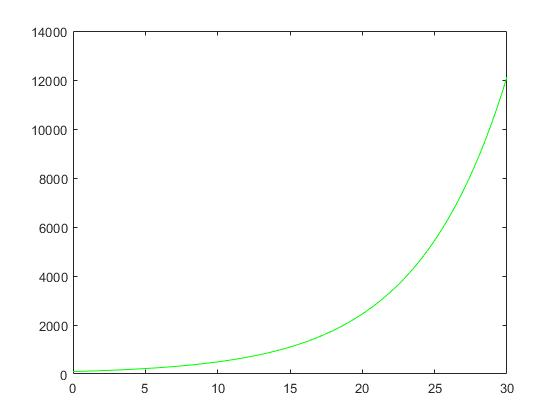
\includegraphics[width=0.5\textwidth]{naloga1.jpg}

\section{2.naloga}

Za Runge-Kutta metodo reda 4 uporabimo sledečo Bučarjevo tabelo

\begin{table}[h]
\begin{tabular}{l|llll}
    &     &     &     &     \\
1/2 & 1/2 &     &     &     \\
1/2 &     & 1/2 &     &     \\
1   &     &     & 1   &     \\ \hline
    & 1/6 & 2/6 & 2/6 & 1/6
\end{tabular}
\end{table}
Rezultati, ki jih dobimo so z Eulerjevo metodo bolj točni, če je korak večji ($1/10$), kot rezultati ki jih dobimo z BDF. Pri manjših korakih pa je BDF metoda bolj točna.

\section{3.naloga}

Za Runge-Kutta metodo reda 4 uporabimo enako tabelo kot v nalogi $2$. Rezultati, ki jih dobimo v tej nalogi so $y(b)= -0.441424015195945$ pri koraku $h=0.1$ in 
$y(b)= -0.422277970368320$ pri koraku $h=0.0.5$.

Zraven dobimo še sledeči graf

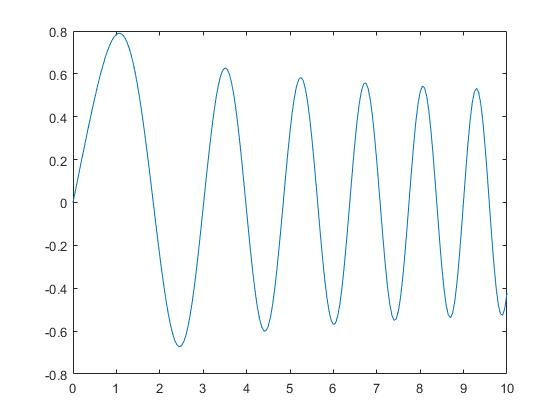
\includegraphics[width=0.5\textwidth]{naloga3.jpg}

\end{document}